\documentclass[10pt]{report}
\usepackage[a4paper]{geometry}
\usepackage[myheadings]{fullpage}
\usepackage{fancyhdr}
\usepackage{lastpage}
\usepackage{graphicx, wrapfig, subcaption, setspace, booktabs}
\usepackage[T1]{fontenc}
\usepackage[font=small, labelfont=bf]{caption}
\usepackage{fourier}
\usepackage[protrusion=true, expansion=true]{microtype}
\usepackage[english]{babel}
\usepackage{sectsty}
\usepackage{url}
\usepackage{amsmath}
\newcommand{\HRule}[1]{\rule{\linewidth}{#1}}
\onehalfspacing
\setcounter{tocdepth}{5}
\setcounter{secnumdepth}{5}
\pagestyle{fancy}
\fancyhf{}
\setlength\headheight{15pt}
%\fancyhead[L]{Group No: 12}
%\fancyhead[R]{Pattern Recognition}
%\fancyfoot[R]{Page \thepage\ of \pageref{LastPage}}


\begin{document}
\title{ \normalsize \textsc{CS6690 : Pattern Recognition}
		\\ [2.0cm]\HRule{0.5pt} \\
        \LARGE \textbf{\uppercase{Assignment 2}}
		\HRule{2pt} \\ [0.5cm]
		\normalsize \today \vspace*{5\baselineskip}}
\date{}
\author{Group No : 12 \\ Kanti Kumari and Sweta Kumari \\Indian Institute of Technology Madras }
\maketitle
%\tableofcontents
\newpage
\sectionfont{\scshape}


\section{Bayesian Classifier}
It is a statistical classification model which classifies the data points based on the probability of the class which it belongs to using mean and covariance of the classes. This technique is based on Bayes' theorem and it calculates the likelihood of data points using Gaussian density function.\\
In the terms of difference between Bayes' and Naive Bayes classifiers, Naive Bayes' assumes independence among the feature vectors while Bayes' does not.
Following are the cases which were used for classification of different types of provided datasets :
\begin{enumerate}
\item Bayesian classification model with same Covariance matrix for each class.
\item Bayesian classification model with different Covariance matrix for each class.
\item Naive Bayes classification model with covariance as $\sigma^2$*I.
\item Naive Bayes classification model with same covariance matrix for each class. 
\item Naive Bayes classification model with different covariance matrix for each class. 
\end{enumerate}
                       
\section{Results}
\begin{figure}[!htb]
\minipage{0.5\textwidth}
  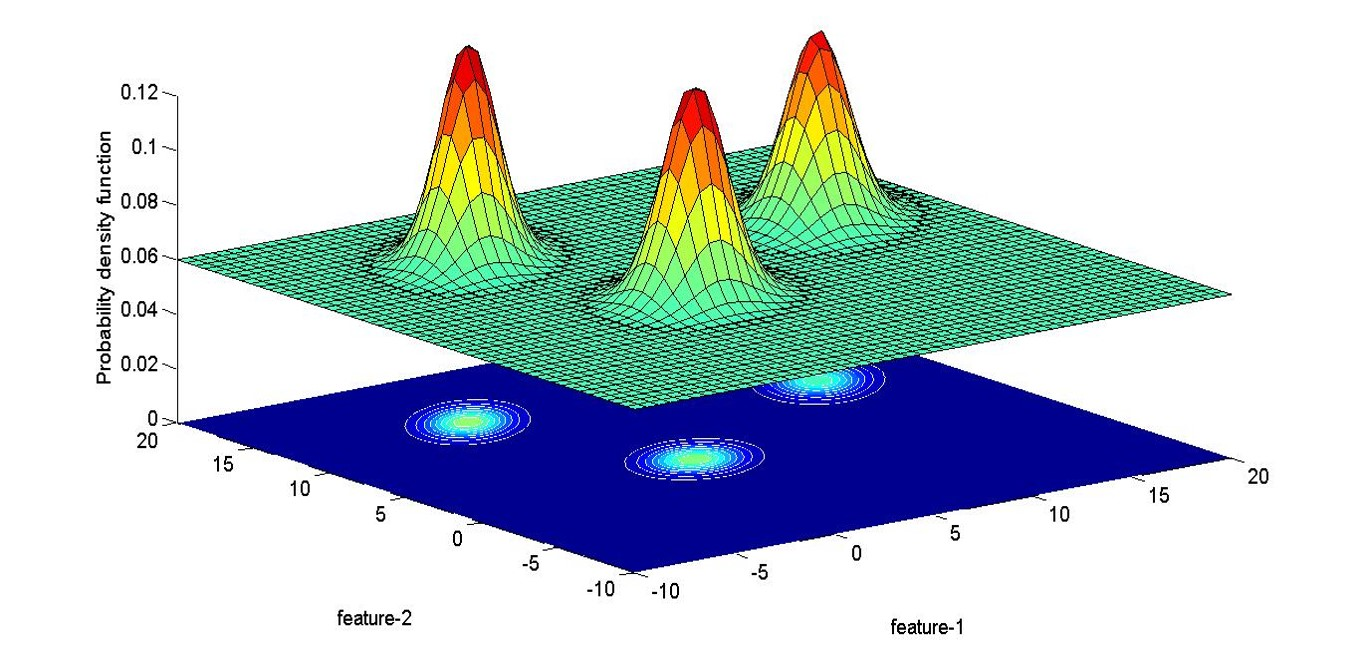
\includegraphics[width=\linewidth]{ls_pdf_con.jpg}
\endminipage\hfill
\minipage{0.5\textwidth}
  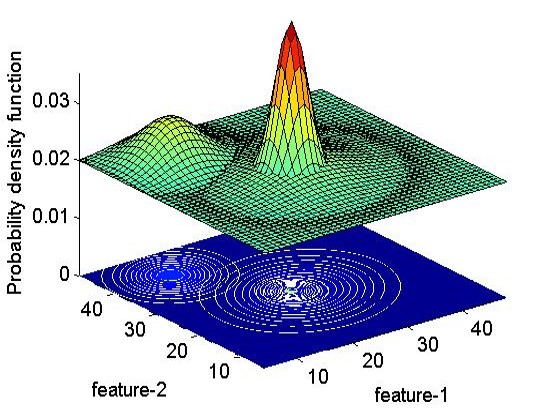
\includegraphics[width=\linewidth]{nls_pdf_con.jpg}
\endminipage\hfill
\caption{PDF (Gaussians) and their contours (constant density curves) for linearly (left) and non-linearly separable data(right).}
\end{figure}

\begin{figure}
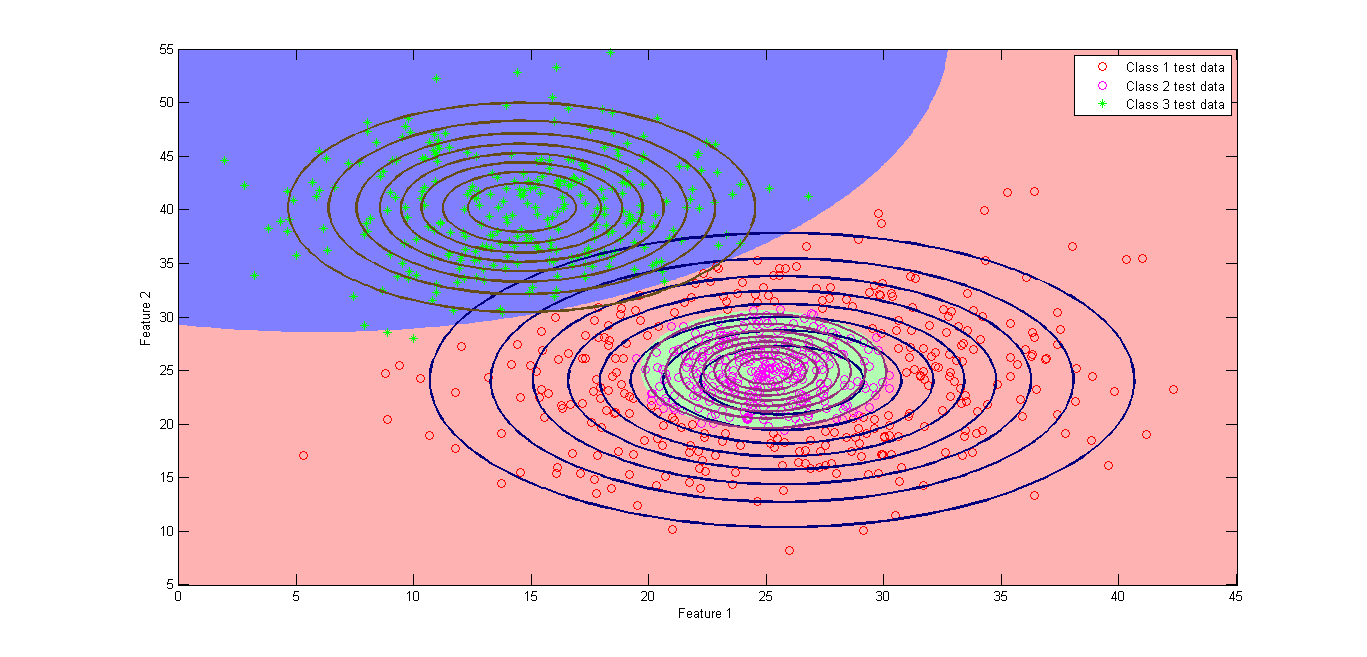
\includegraphics[width=\linewidth]{des_con_.png}
\caption{Descision boundary, decision surface and constant density curve for non linearly separable data.}
\end{figure}

\begin{figure}[!htb]
\minipage{0.5\textwidth}
  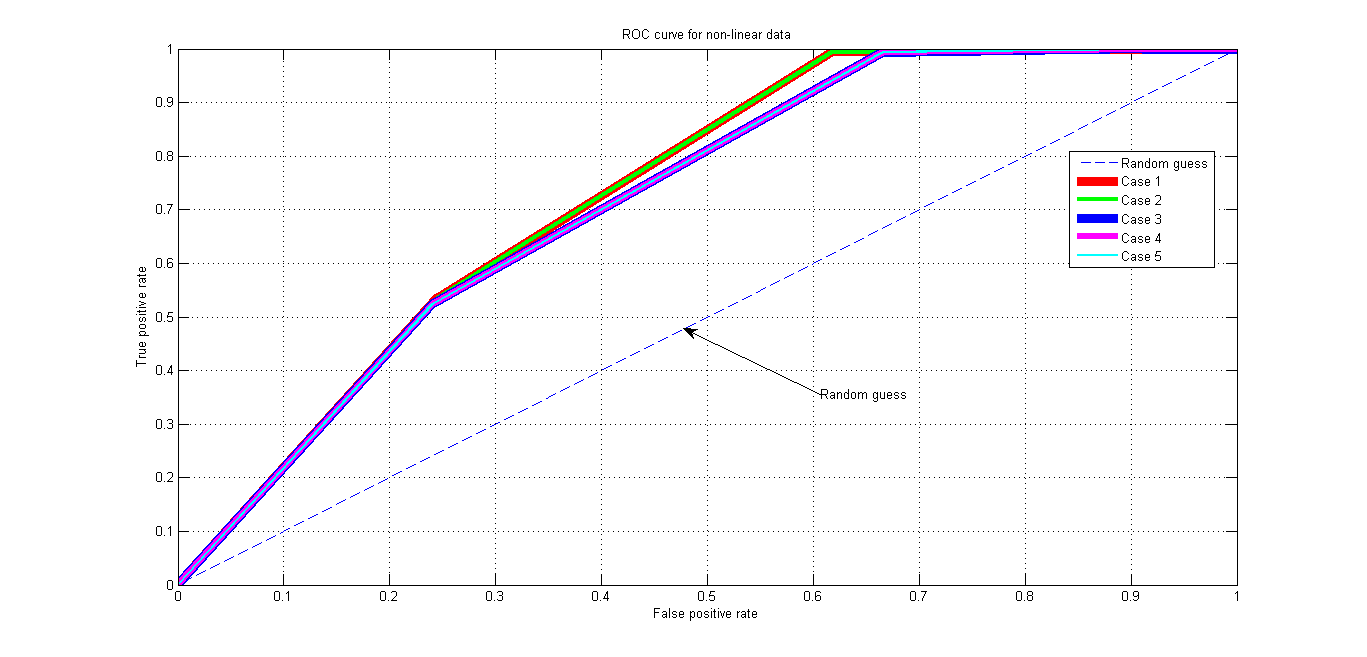
\includegraphics[width=\linewidth]{roc_nonlin.png}
\endminipage\hfill
\minipage{0.5\textwidth}
  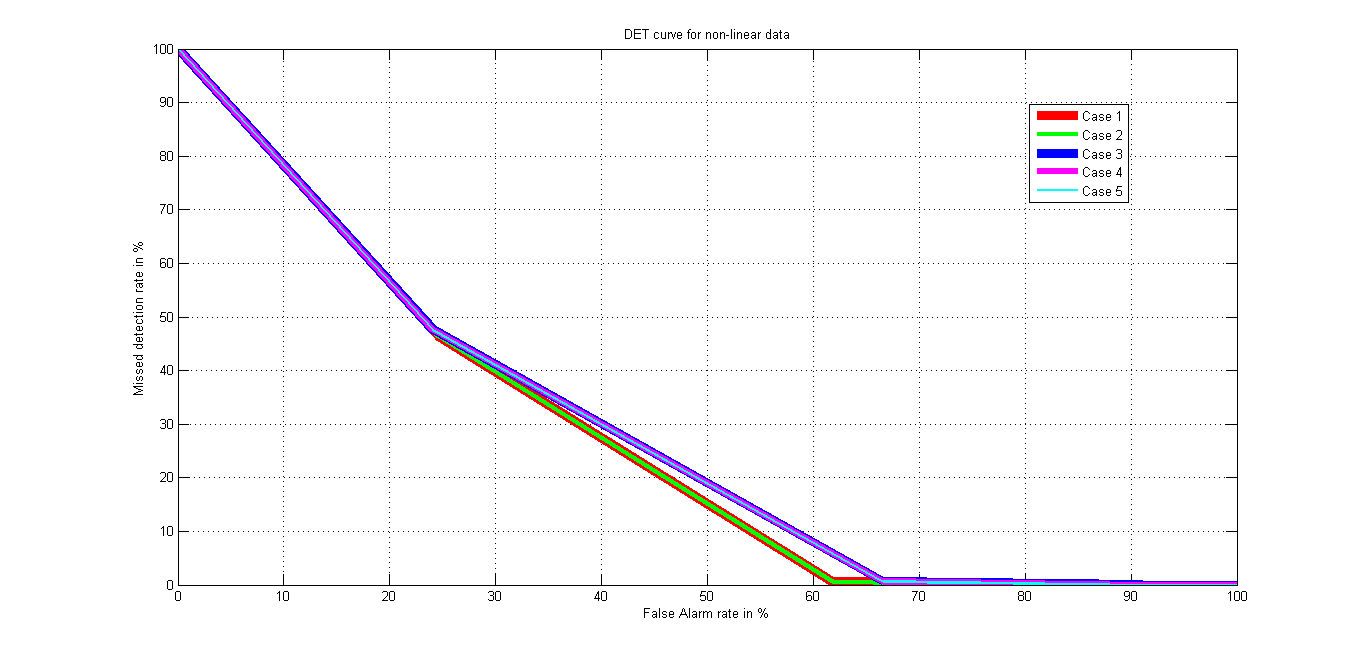
\includegraphics[width=\linewidth]{det_nonlin.png}
\endminipage\hfill
\caption{ROC and DET curve for non-linearly separable data.}
\end{figure}

\begin{figure}[!htb]
\minipage{0.5\textwidth}
  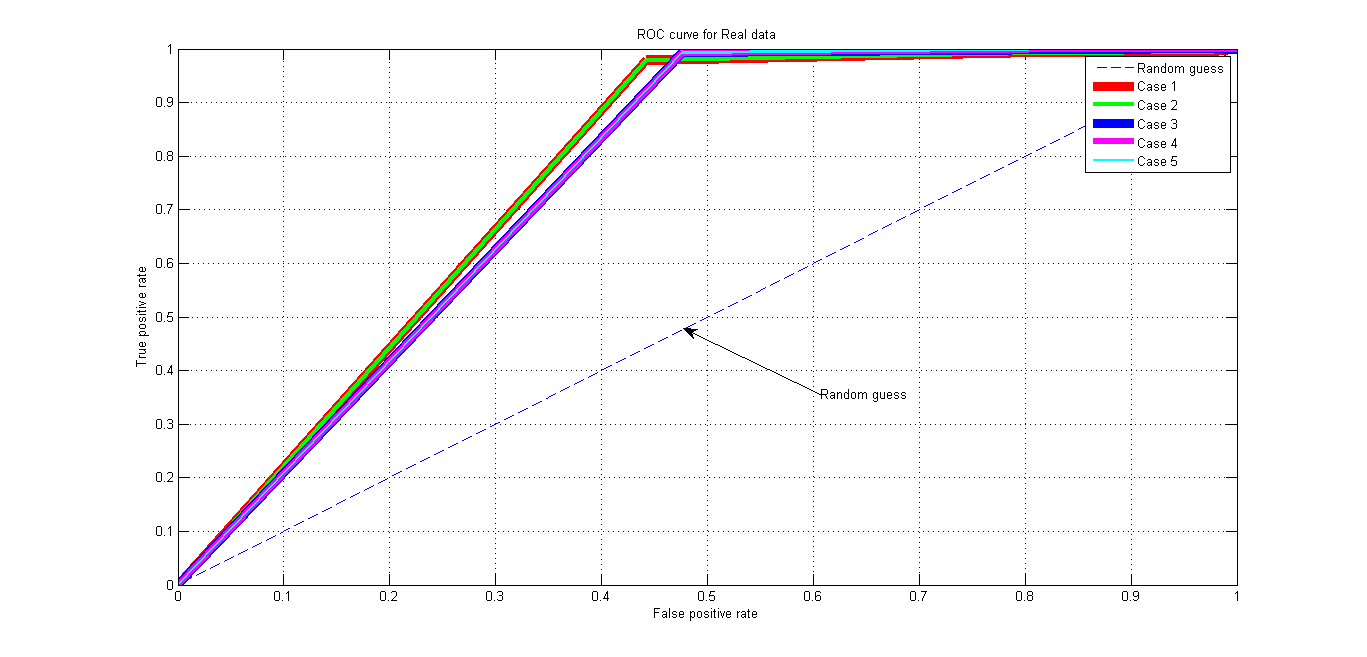
\includegraphics[width=\linewidth]{roc_real.png}
\endminipage\hfill
\minipage{0.5\textwidth}
  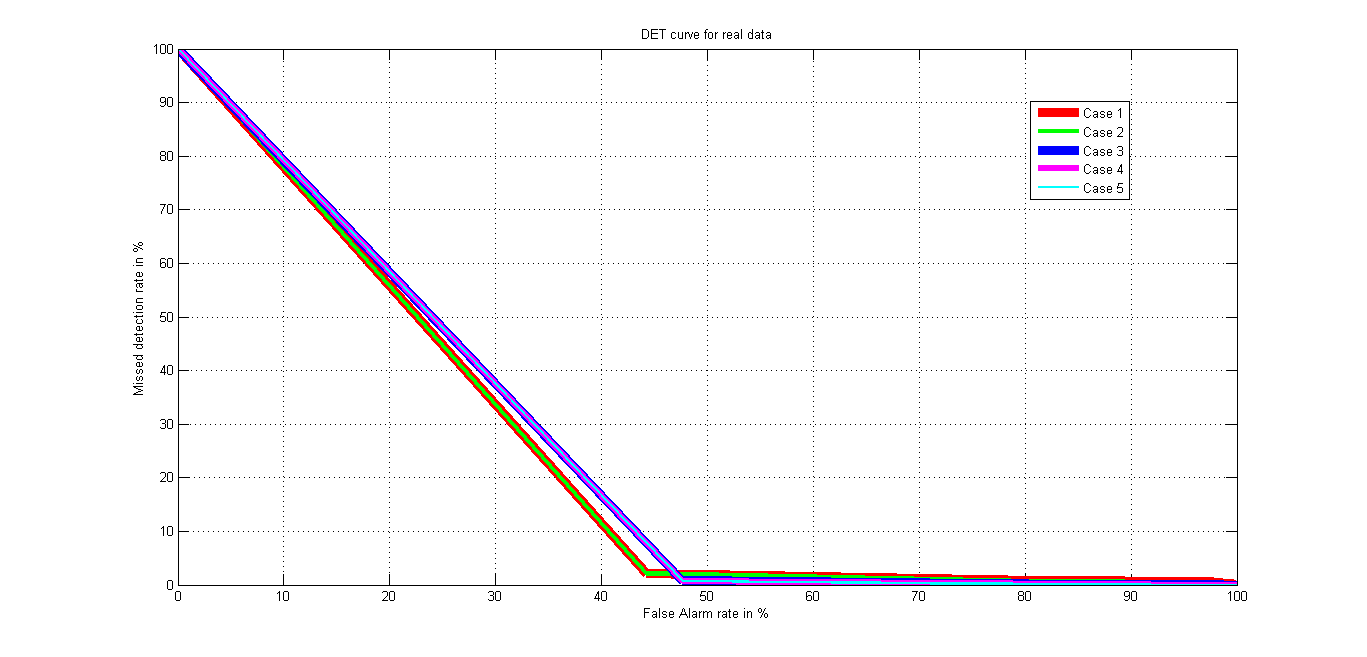
\includegraphics[width=\linewidth]{det_real.png}
\endminipage\hfill
\caption{ROC and DET curve for real data.}
\end{figure}

\begin{figure}[!htb]
\minipage{0.5\textwidth}
  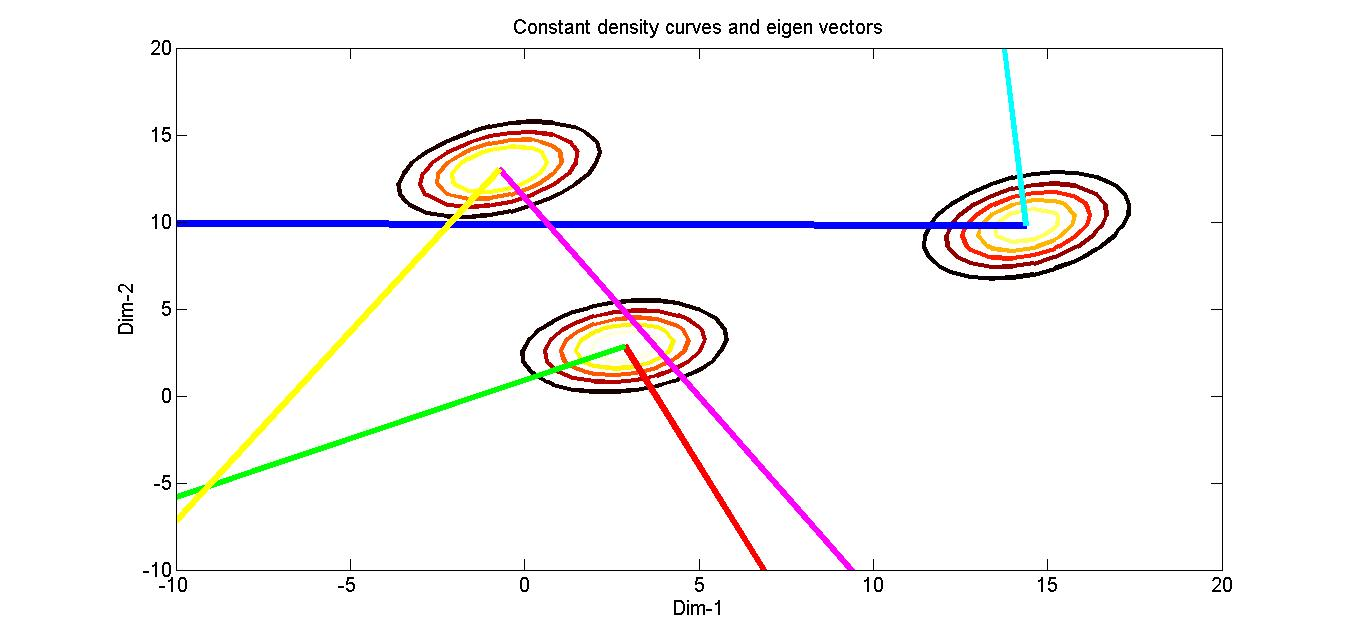
\includegraphics[width=\linewidth]{eigen_lin.jpg}
\endminipage\hfill
\minipage{0.5\textwidth}
  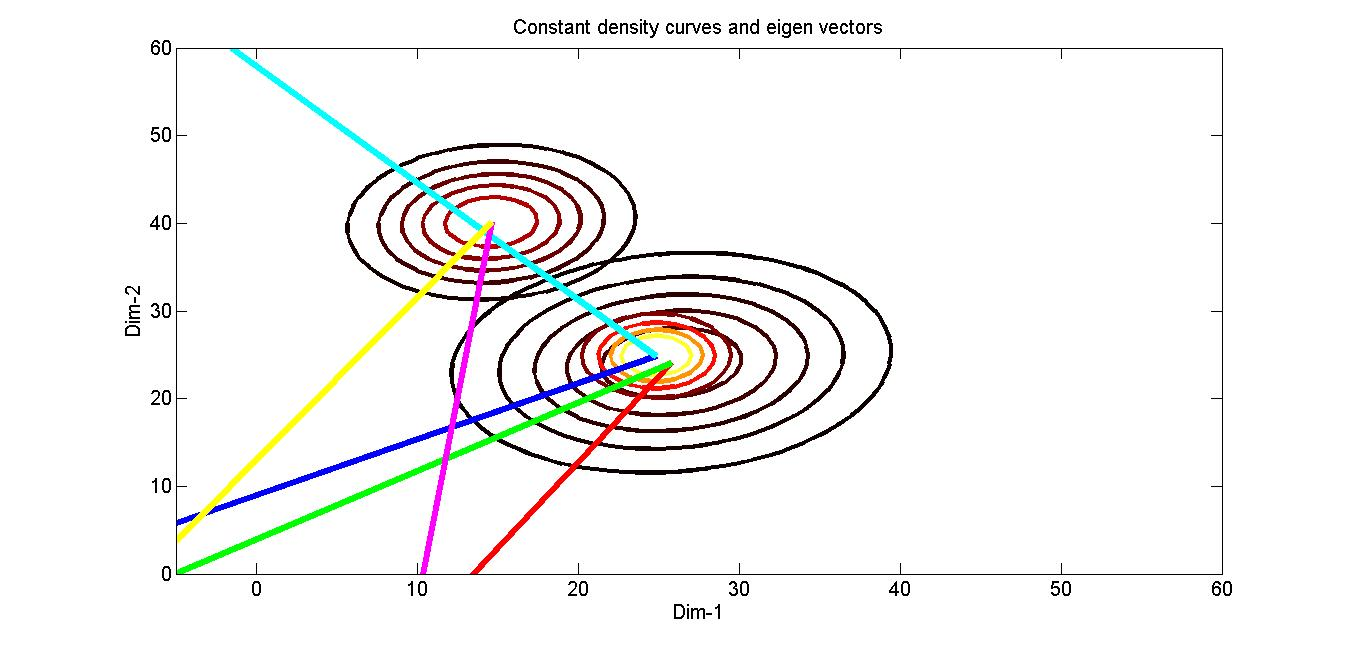
\includegraphics[width=\linewidth]{eigen_nonlin.jpg}
\endminipage\hfill
\caption{Constant density curves with eigenvectors for linear and non-linear data respectively.}
\end{figure}

\begin{figure}[!htb]
\minipage{0.5\textwidth}
  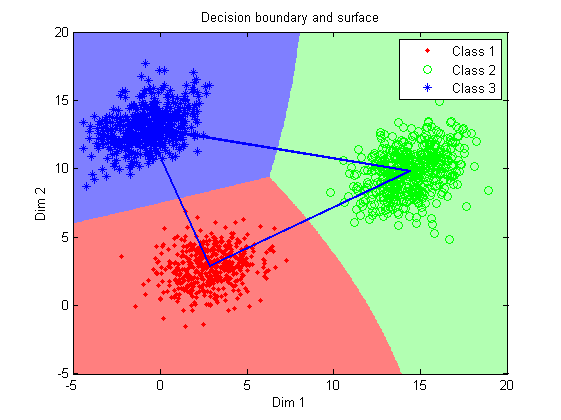
\includegraphics[width=\linewidth]{des_lin.png}
\endminipage\hfill
\minipage{0.5\textwidth}
  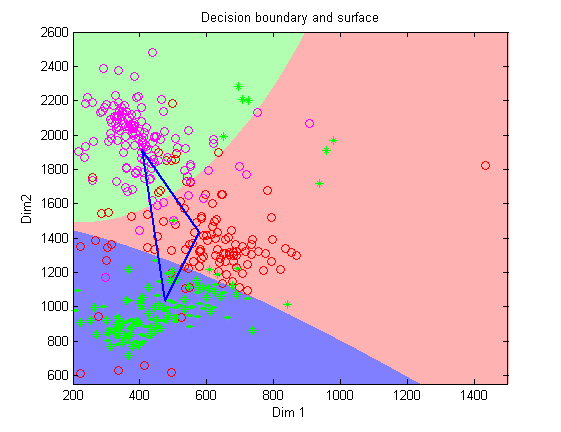
\includegraphics[width=\linewidth]{des_real.png}
\endminipage\hfill
\caption{Decision Boundary and decision surface for linear and real data.}
\end{figure}
\begin{figure}[!htb]
\minipage{0.5\textwidth}
  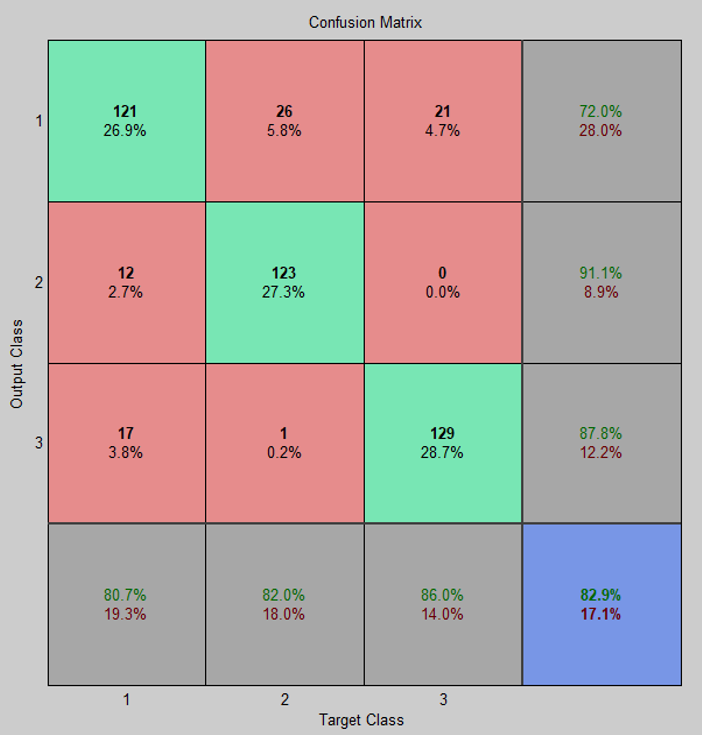
\includegraphics[width=\linewidth]{conf_real_case2.png}
\endminipage\hfill
\minipage{0.5\textwidth}
  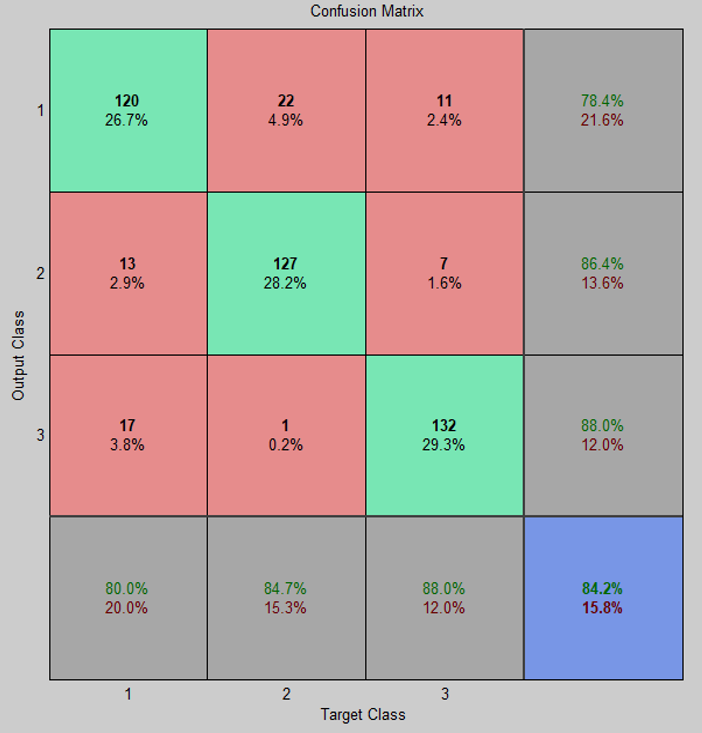
\includegraphics[width=\linewidth]{conf_real_case3.png}
\endminipage\hfill
\caption{Confusion matrix for real data in Case 2 and 3 respectively.}
\end{figure}

\begin{figure}
\begin{center}
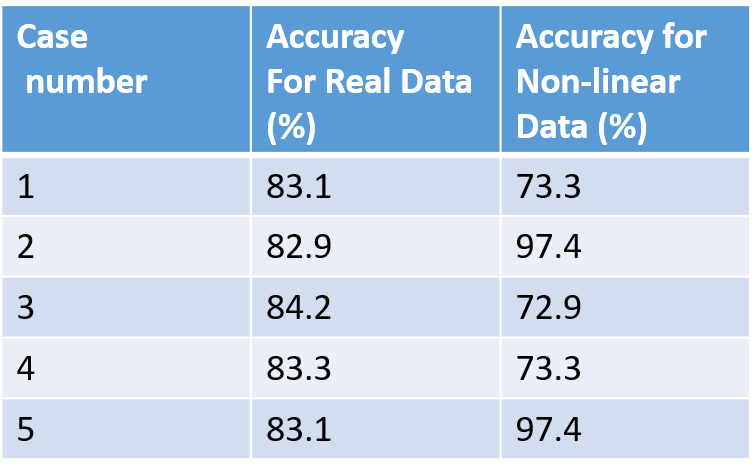
\includegraphics[scale=0.5]{table.png}
\caption{Case-wise Accuracy comparison table for real and non-linear data.}
\end{center}
\end{figure}
\newpage
\newpage
\newpage
\newpage
\newpage
\newpage
\section{Conclusion}
After performing experiment with all of the given cases for different types of provided datasets, we observed accuracy as :
\begin{enumerate}
\item For linear dataset: Accuracy were same for all cases.
\item For non-linear dataset: 
	\begin{enumerate}
		\item Accuracy were same in case 2 and 5 (highest).
    	\item Accuracy were same in case 1, 3 and 4 (lowest).
     \end{enumerate}
\item For real dataset: 
	\begin{enumerate}
		\item Accuracy were same in case 1 and 5.
    	\item Accuracy were different in case 2, 3 and 4.    
     \end{enumerate}
\end{enumerate}
\end{document}

